\documentclass[aspectratio=169, lualatex, handout]{beamer}
\makeatletter\def\input@path{{theme/}}\makeatother\usetheme{cipher}

\title{Applied Cryptography - 2.8: Zero-Knowledge Proofs}
\author{Nadim Kobeissi}
\subject{TODO}
\keywords{TODO}
\institute{American University of Beirut}
\instituteimage{images/aub_white.png}
\date{\today}
\coversubtitle{CMPS 297AD/396AI\\Fall 2025}
\coverpartname{Part 2: Real-World Cryptography}
\covertopicname{2.8: Zero-Knowledge Proofs}
\coverwebsite{https://appliedcryptography.page}

\begin{document}
\begin{frame}[plain]
	\titlepage
\end{frame}

\section{Introduction}

\begin{frame}{Zero-knowledge proofs: magic, but real}
	\begin{columns}[c]
		\begin{column}{0.5\textwidth}
			\textbf{Imagine this scenario:}
			\begin{itemize}
				\item I claim to know the password to a secret vault
				\item You need to verify I really know it
				\item But I don't want to tell you the password!
			\end{itemize}
			\textbf{Seems impossible?}
			\begin{itemize}
				\item How can I prove knowledge without revealing it?
				\item This is the magic of zero-knowledge proofs
			\end{itemize}
		\end{column}
		\begin{column}{0.5\textwidth}
			\begin{block}{Zero-knowledge property}
				A proof that reveals \textbf{nothing} except the truth of the statement being proven
			\end{block}
			\vspace{0.5em}
			\begin{alertblock}{The paradox}
				Convince you completely while teaching you nothing
			\end{alertblock}
		\end{column}
	\end{columns}
\end{frame}

\begin{frame}{What makes zero-knowledge proofs special?}
	\textbf{Traditional proof:}
	\begin{itemize}
		\item ``Here's my password: \texttt{hunter2}''
		\item You learn the secret itself
		\item You could now impersonate me
	\end{itemize}
	\textbf{Zero-Knowledge proof:}
	\begin{itemize}
		\item ``I'll convince you I know the password''
		\item You learn \textit{only} that I know it
		\item You gain no ability to prove it yourself
		\item You can't replay my proof to others
	\end{itemize}
\end{frame}

\begin{frame}{The three zero-knowledge properties}
	\begin{block}{1. Completeness}
		If the statement is true, an honest prover can convince an honest verifier
	\end{block}
	\begin{block}{2. Soundness}
		If the statement is false, no cheating prover can convince an honest verifier (except with negligible probability)
	\end{block}
	\begin{block}{3. Zero-Knowledge}
		The verifier learns nothing beyond the validity of the statement
	\end{block}
	\vspace{0.25em}
	\begin{center}
		\textbf{These three properties together create the ``magic''}
	\end{center}
\end{frame}

\begin{frame}{Also, knowledge soundness}
	\begin{columns}[c]
		\begin{column}{0.5\textwidth}
			\begin{itemize}
				\item \textbf{Regular Soundness:}
				      \begin{itemize}
					      \item Prevents false statements from being proved
					      \item ``Can't prove something that's false''
					      \item Example: Can't prove $g^a = X$ if no such $a$ exists
					      \item Weaker guarantee
				      \end{itemize}
				\item \textbf{Sufficient when:}
				      \begin{itemize}
					      \item Only care about statement validity
					      \item Don't need witness extraction
					      \item Simple yes/no verification
				      \end{itemize}
			\end{itemize}
		\end{column}
		\begin{column}{0.5\textwidth}
			\begin{itemize}
				\item \textbf{Knowledge Soundness:}
				      \begin{itemize}
					      \item If prover succeeds, they \textit{know} a witness
					      \item ``Can extract the witness from successful prover''
					      \item Example: Can extract the actual value $a$
					      \item Stronger guarantee
				      \end{itemize}
				\item \textbf{Essential when:}
				      \begin{itemize}
					      \item Building signatures schemes
					      \item Proving knowledge credentials
					      \item Composition with other protocols
				      \end{itemize}
			\end{itemize}
		\end{column}
	\end{columns}
\end{frame}

\begin{frame}{Example: Proving Knowledge of a Private Key}
	\begin{columns}[c]
		\begin{column}{0.5\textwidth}
			\textbf{The Setup:}
			\begin{itemize}
				\item Public key: $A = g^{a}$
				\item I claim to know $a$
				\item But revealing $a$ would compromise security
			\end{itemize}
			\textbf{Zero-Knowledge Solution:}
			\begin{enumerate}
				\item Interactive protocol
				\item Multiple rounds of challenges
				\item Statistically convincing
				\item Reveals nothing about $a$
			\end{enumerate}
		\end{column}
		\begin{column}{0.5\textwidth}
			\begin{alertblock}{Can't prove to others}
				After our interaction:
				\begin{itemize}
					\item You're 100\% convinced I know $a$
					\item You've learned nothing about $a$
					\item You can't prove to others that I know it
				\end{itemize}
			\end{alertblock}
			\vspace{0.5em}
			\begin{exampleblock}{No ``trace'' or ``evidence''}
				The interaction leaves no transferable evidence
			\end{exampleblock}
		\end{column}
	\end{columns}
\end{frame}

\begin{frame}{Schnorr Identification Protocol}
	\vspace{-1.5cm}
	\begin{center}\resizebox{0.8\textwidth}{!}{
			\begin{msc}{}
				\setmscvalues{small}
				\drawframe{none}
				\setlength{\instdist}{8cm}
				\setlength{\instwidth}{2cm}
				\declinst{prover}{}{Prover}
				\declinst{verifier}{}{Verifier}
				\action*{$\begin{array}{l}
							\text{Knows generator}~g         \\
							\text{Knows prime}~n             \\
							\text{Knows secret}~a            \\
							y \twoheadleftarrow \mathbb{Z}_n \\
							Y = g^y
						\end{array}$}{prover}
				\action*{$\begin{array}{l}
							\text{Knows generator}~g                 \\
							\text{Knows prime}~n                     \\
							\text{Knows prover's public key}~A = g^a \\
						\end{array}$}{verifier}
				\nextlevel[7]
				\mess{$Y$}{prover}{verifier}
				\nextlevel[1]
				\action*{$c \twoheadleftarrow \mathbb{Z}_n$}{verifier}
				\nextlevel[2]
				\mess{$c$}{verifier}{prover}
				\nextlevel[1]
				\action*{$r = (y + ca) \bmod n$}{prover}
				\nextlevel[2]
				\mess{$r$}{prover}{verifier}
				\nextlevel[1]
				\action*{$g^r \overset{?}{\equiv} Y \cdot A^c$}{verifier}
				\nextlevel[2]
			\end{msc}
		}\end{center}
\end{frame}

\begin{frame}{Schnorr Identification Protocol}
	\begin{columns}[c]
		\begin{column}{0.6\textwidth}
			\begin{itemize}
				\item \textbf{Interactive proof:} Multiple rounds of communication
				\item \textbf{Commitment phase:} Prover commits to random $Y = g^y$
				\item \textbf{Challenge phase:} Verifier sends random challenge $c$
				\item \textbf{Response phase:} Prover computes $r = y + ca$
				\item \textbf{Verification:} Check if $g^r = Y \cdot A^c$
				\item \textbf{Zero-knowledge property:} $r$ reveals nothing about $a$ due to random masking by $y$
				\item \textbf{Soundness:} Without knowing $a$, prover can't answer random challenges correctly
			\end{itemize}
		\end{column}
		\begin{column}{0.4\textwidth}
			\vspace{-1.5cm}
			\begin{center}\resizebox{1\textwidth}{!}{
					\begin{msc}{}
						\setmscvalues{small}
						\drawframe{none}
						\setlength{\instdist}{8cm}
						\setlength{\instwidth}{2cm}
						\declinst{prover}{}{Prover}
						\declinst{verifier}{}{Verifier}
						\action*{$\begin{array}{l}
									\text{Knows generator}~g         \\
									\text{Knows prime}~n             \\
									\text{Knows secret}~a            \\
									y \twoheadleftarrow \mathbb{Z}_n \\
									Y = g^y
								\end{array}$}{prover}
						\action*{$\begin{array}{l}
									\text{Knows generator}~g                 \\
									\text{Knows prime}~n                     \\
									\text{Knows prover's public key}~A = g^a \\
								\end{array}$}{verifier}
						\nextlevel[7]
						\mess{$Y$}{prover}{verifier}
						\nextlevel[1]
						\action*{$c \twoheadleftarrow \mathbb{Z}_n$}{verifier}
						\nextlevel[2]
						\mess{$c$}{verifier}{prover}
						\nextlevel[1]
						\action*{$r = (y + ca) \bmod n$}{prover}
						\nextlevel[2]
						\mess{$r$}{prover}{verifier}
						\nextlevel[1]
						\action*{$g^r \overset{?}{\equiv} Y \cdot A^c$}{verifier}
						\nextlevel[2]
					\end{msc}
				}\end{center}
		\end{column}
	\end{columns}
\end{frame}

\begin{frame}{The verifier learned literally nothing new}
	\begin{columns}[c]
		\begin{column}{0.55\textwidth}
			\begin{itemize}
				\item After the protocol, you're convinced I know the secret
				\item But you can't convince anyone else!
				\item Why? The transcript looks identical to \textbf{something you could have generated alone}
				\item \textbf{The simulation argument:}
				      \begin{itemize}
					      \item You could have picked $r$ and $c$ randomly
					      \item Then computed $Y = g^r / A^c$
					      \item This produces a valid-looking transcript!
					      \item No way to distinguish from real interaction
				      \end{itemize}
			\end{itemize}
		\end{column}
		\begin{column}{0.45\textwidth}
			\resizebox{0.8\textwidth}{!}{%
				\begin{minipage}{\textwidth}
					\begin{alertblock}{Self-generated transcripts}
						For any challenge $c$ and response $r$:
						\begin{itemize}
							\item Set $Y = g^r / A^c$
							\item Now $(Y, c, r)$ is a valid transcript
							\item Indistinguishable from real protocol
							\item Real interaction: Prover knows secret
							\item Simulated transcript: No secret needed
							\item Both look exactly the same!
							\item This is what makes it ``zero-knowledge''
						\end{itemize}
					\end{alertblock}
				\end{minipage}%
			}
		\end{column}
	\end{columns}
\end{frame}

\begin{frame}{In other words\ldots}
	\begin{center}
		\sslinked{
			\sslibrary{}{schnorr-real}{
				\sslibrarysubroutine{schnorr.transcript}{a}{
					$A := g^a$ \\
					$y \twoheadleftarrow \mathbb{Z}_n$ \\
					$Y := g^y$ \\
					$c \twoheadleftarrow \mathbb{Z}_n$ \\
					$r := (y + ca) \bmod n$ \\
					return $(A, Y, c, r)$
				}{1}
			}{1}
		}{\interchangeable}{
			\sslibrary{}{schnorr-fake}{
				\sslibrarysubroutine{schnorr.transcript}{a}{
					$A := g^a$ \\
					$c \twoheadleftarrow \mathbb{Z}_n$ \\
					$r \twoheadleftarrow \mathbb{Z}_n$ \\
					$Y := g^r \cdot (A^c)^{-1}$ \\
					return $(A, Y, c, r)$
				}{1}
			}{1}
		}
	\end{center}
\end{frame}

\begin{frame}{Quick reminder: What does $x^{-1}$ mean?}
	\begin{columns}[c]
		\begin{column}{0.5\textwidth}
			\textbf{In modular arithmetic:}
			\begin{itemize}
				\item $x^{-1}$ is the \textbf{modular inverse} of $x$
				\item It's the number that, when multiplied by $x$, gives 1
				\item $x \cdot x^{-1} \equiv 1 \pmod{n}$
			\end{itemize}
			\textbf{Example:}
			\begin{itemize}
				\item If $x = 3$ and $n = 7$
				\item Then $x^{-1} = 5$ because $3 \cdot 5 = 15 \equiv 1 \pmod{7}$
			\end{itemize}
		\end{column}
		\begin{column}{0.5\textwidth}
			\textbf{In group elements:}
			\begin{itemize}
				\item If $A = g^a$, then $A^{-1} = g^{-a}$
				\item $A \cdot A^{-1} = g^a \cdot g^{-a} = g^{a-a} = g^0 = 1$
				\item It's the element that ``cancels out'' $A$
			\end{itemize}
			\begin{alertblock}{Key property}
				$(A^c)^{-1} = A^{-c}$ \\
				This is why we can rewrite expressions!
			\end{alertblock}
		\end{column}
	\end{columns}
\end{frame}

\begin{frame}{Proof of indistinguishability}{Step 1}
	\begin{columns}[c]
		\begin{column}{0.5\textwidth}
			\begin{itemize}[<+->]
				\item We can rearrange things so that $c$ is chosen first.
			\end{itemize}
		\end{column}
		\begin{column}{0.5\textwidth}
			\begin{center}
				\sslibrary{}{schnorr-real}{
					\sslibrarysubroutine{schnorr.transcript}{a}{
						$A := g^a$ \\
						$c \twoheadleftarrow \mathbb{Z}_n$ \\
						\hl{$y \twoheadleftarrow \mathbb{Z}_n$} \\
						$r := (y + ca) \bmod n$ \\
						\hl{$Y := g^y$} \\
						return $(A, Y, c, r)$
					}{1}
				}{1}
			\end{center}
		\end{column}
	\end{columns}
\end{frame}

\begin{frame}{Proof of indistinguishability}{Step 2}
	\begin{columns}[c]
		\begin{column}{0.5\textwidth}
			\begin{itemize}[<+->]
				\item $r$ is essentially a OTP encryption of plaintext $ca$ under key $y$, using a variant of OTP with addition $\bmod\ n$.
				\item We can achieve the same distribution by choosing $r$ uniformly and solving for $y$.
			\end{itemize}
		\end{column}
		\begin{column}{0.5\textwidth}
			\begin{center}
				\sslibrary{}{schnorr-real}{
					\sslibrarysubroutine{schnorr.transcript}{a}{
						$A := g^a$ \\
						$c \twoheadleftarrow \mathbb{Z}_n$ \\
						\hl{$r \twoheadleftarrow \mathbb{Z}_n$} \\
						\hl{$y := (r - ca) \bmod n$} \\
						$Y := g^y$ \\
						return $(A, Y, c, r)$
					}{1}
				}{1}
			\end{center}
		\end{column}
	\end{columns}
\end{frame}

\begin{frame}{Proof of indistinguishability}{Step 3}
	\begin{columns}[c]
		\begin{column}{0.5\textwidth}
			\begin{itemize}[<+->]
				\item $Y$ is computed as
				      \begin{align*}
					      Y & = g^y                       \\
					        & = g^{r-ca}                  \\
					        & = g^{r} \cdot (g^{ca})^{-1} \\
					        & = g^{r} \cdot (A^{c})^{-1}
				      \end{align*}
				\item By rewriting $Y$ in this way, the private exponent $a$ is no longer needed.
			\end{itemize}
		\end{column}
		\begin{column}{0.5\textwidth}
			\begin{center}
				\sslibrary{}{schnorr-fake}{
					\sslibrarysubroutine{schnorr.transcript}{a}{
						$A := g^a$ \\
						$c \twoheadleftarrow \mathbb{Z}_n$ \\
						$r \twoheadleftarrow \mathbb{Z}_n$ \\
						$y := (r - ca) \bmod n$ \\
						\hl{$Y := g^r \cdot (A^c)^{-1}$} \\
						return $(A, Y, c, r)$
					}{1}
				}{1}
			\end{center}
		\end{column}
	\end{columns}
\end{frame}

\begin{frame}{Understanding the exponent manipulation}
	\begin{columns}[c]
		\begin{column}{0.5\textwidth}
			\textbf{Why does $g^{r-ca} = g^r \cdot (g^{ca})^{-1}$?}
			\begin{itemize}
				\item Recall the exponent rule: $g^{x-y} = \frac{g^x}{g^y}$
				\item In group notation, division is multiplication by inverse
				\item So $\frac{g^x}{g^y} = g^x \cdot (g^y)^{-1}$
			\end{itemize}
			\textbf{Step by step:}
			\begin{enumerate}
				\item $g^{r-ca} = \frac{g^r}{g^{ca}}$ (exponent rule)
				\item $\frac{g^r}{g^{ca}} = g^r \cdot (g^{ca})^{-1}$ (division = multiply by inverse)
			\end{enumerate}
		\end{column}
		\begin{column}{0.5\textwidth}
			\begin{exampleblock}{Concrete example}
				Let's use regular numbers to see why:
				\begin{itemize}
					\item If $g = 2$, $r = 7$, $ca = 3$
					\item $2^{7-3} = 2^4 = 16$
					\item $2^7 \cdot (2^3)^{-1} = 128 \cdot \frac{1}{8} = 16$ \mycheckmark
				\end{itemize}
			\end{exampleblock}
			\vspace{0.5em}
			\begin{alertblock}{Observe how\ldots}
				This manipulation lets us separate the secret exponent $a$ from the computation!
			\end{alertblock}
		\end{column}
	\end{columns}
\end{frame}

\begin{frame}{In other words\ldots}
	\begin{center}
		\sslinked{
			\sslibrary{}{schnorr-real}{
				\sslibrarysubroutine{schnorr.transcript}{a}{
					$A := g^a$ \\
					$y \twoheadleftarrow \mathbb{Z}_n$ \\
					$Y := g^y$ \\
					$c \twoheadleftarrow \mathbb{Z}_n$ \\
					$r := (y + ca) \bmod n$ \\
					return $(A, Y, c, r)$
				}{1}
			}{1}
		}{\interchangeable}{
			\sslibrary{}{schnorr-fake}{
				\sslibrarysubroutine{schnorr.transcript}{a}{
					$A := g^a$ \\
					$c \twoheadleftarrow \mathbb{Z}_n$ \\
					$r \twoheadleftarrow \mathbb{Z}_n$ \\
					$Y := g^r \cdot (A^c)^{-1}$ \\
					return $(A, Y, c, r)$
				}{1}
			}{1}
		}
	\end{center}
\end{frame}

\begin{frame}{A parable}
	\begin{center}
		\vfill
		\large
		\textit{\rmfamily ``King Richard decides to hold an archery competition to identify the best archer in the land. He constructs a long wooden wall, with many targets painted on it. During the competition, he is stunned as Robin Hood stands 100 meters away from the wall and fires one arrow into the center of each of the targets. Of course, Robin Hood is declared the winner.''}
		\vfill
	\end{center}
\end{frame}

\begin{frame}{A parable}
	\begin{center}
		\vfill
		\large
		\textit{\rmfamily ``Later that day, the Sheriff of Nottingham arrives at the King's castle. The King describes Robin Hood's exceptional performance, pointing to the arrows still in the targets. The Sheriff is not impressed. “Robin Hood is a fraud and a liar. Those arrows prove nothing,” he says. He takes his own bow and fires a series of arrows into blank parts of the wall. He finds a bucket of paint and paints a target around each of his arrows. ``See,'' he says again, ``arrows in targets prove nothing!''''}
		\vfill
	\end{center}
\end{frame}

\begin{frame}{Another parable}
	\begin{center}
		\vfill
		\large
		\textit{\rmfamily ``Alice, whose public key is $A = g^a$, contacts Bob and uses Schnorr's protocol to prove that she knows the secret key $a$. Bob is convinced that he is talking to Alice, and he writes down everything he sees: $(A, Y, c, r)$.''}
		\vfill
	\end{center}
\end{frame}

\begin{frame}{Another parable}
	\begin{center}
		\vfill
		\large
		\textit{\rmfamily ``Later that day, Charlie arrives at Bob's house. Bob mentions that he talked to Alice earlier in the day, and he shows Charlie the accepting transcript $(A,Y,c,r)$. ``That proves nothing,'' says Charlie, and he proceeds to generate his own accepting transcript $(A,Y',c',r')$, even though he doesn't know $a$.''}
		\vfill
	\end{center}
\end{frame}

\section{Sigma Protocols}

\begin{frame}{ZK can scale to entire systems}{Reminder}
	\begin{columns}[c]
		\begin{column}{0.6\textwidth}
			\begin{itemize}[<+->]
				\item As seen previously, you can build entire \textbf{zero-knowledge protocols}, not just primitives that prove knowledge of certain numbers.
				\item ``Zero-knowledge virtual machines'' where you can execute
				      an entire program that runs as a zero-knowledge proof.
				\item ZKP battleship game: server proves to the players that its
				      output to their battleship guesses is correct, without revealing any
				      additional information (e.g. ship location).
			\end{itemize}
		\end{column}
		\begin{column}{0.4\textwidth}
			\imagewithcaption{battleship.jpg}{Battleship board game. Source: Hasbro}
		\end{column}
	\end{columns}
\end{frame}

\begin{frame}{Beyond authentication: the power of zero-knowledge}
	\begin{center}
		\textbf{Zero-knowledge is not limited to proving identity!}
	\end{center}
	\vspace{0.25em}
	\begin{columns}[c]
		\begin{column}{0.6\textwidth}
			\begin{itemize}
				\item \textbf{Can prove statements like:}
				      \begin{itemize}
					      \item \textit{``I know a solution to this Sudoku puzzle''}
					      \item \textit{``This encrypted value is in range [0, 100]''} (range proofs)
					      \item \textit{``I performed this computation correctly''}
					      \item \ldots without revealing any information!
				      \end{itemize}
			\end{itemize}
		\end{column}
		\begin{column}{0.4\textwidth}
			\begin{itemize}
				\item \textbf{Applications:}
				      \begin{itemize}
					      \item Private transactions (Zcash)
					      \item Anonymous credentials
					      \item Secure voting systems
					      \item Privacy-preserving audits
				      \end{itemize}
			\end{itemize}
		\end{column}
	\end{columns}
\end{frame}

\subsection{Sigma Protocols: High-Level Overview}

\begin{frame}{From Schnorr to Sigma, a general framework}
	\begin{columns}[c]
		\begin{column}{0.5\textwidth}
			\textbf{Schnorr was just the beginning!}
			\begin{itemize}
				\item Schnorr proves: ``I know $a$ such that $g^a = A$''
				\item What if we want to prove other statements?
				\item Enter \textbf{Sigma protocols}: a general framework
			\end{itemize}
			\vspace{0.5em}
			\textbf{The pattern:}
			\begin{itemize}
				\item Public instance: $X$
				\item Private witness: $W$
				\item Relation: $R(X, W) = \text{true}$
			\end{itemize}
		\end{column}
		\begin{column}{0.5\textwidth}
			\begin{exampleblock}{Examples of relations}
				\begin{itemize}
					\item ``I know $a$ such that $g^a = X$''
					      \begin{itemize}
						      \item Witness: $a$
					      \end{itemize}
					\item ``I know $(r, s)$ such that $g^r h^s = X$''
					      \begin{itemize}
						      \item Witness: $(r, s)$
					      \end{itemize}
					\item ``I know a factorization of $X$''
					      \begin{itemize}
						      \item Witness: $(p, q)$ where $X = p \cdot q$
					      \end{itemize}
					\item ``I know a graph coloring for $X$''
					      \begin{itemize}
						      \item Witness: The coloring assignment
					      \end{itemize}
				\end{itemize}
			\end{exampleblock}
		\end{column}
	\end{columns}
\end{frame}

\begin{frame}{Sigma protocol structure}
	\vspace{-1.5cm}
	\begin{center}\resizebox{0.8\textwidth}{!}{
			\begin{msc}{}
				\setmscvalues{small}
				\drawframe{none}
				\setlength{\instdist}{8cm}
				\setlength{\instwidth}{2cm}
				\declinst{prover}{}{Prover}
				\declinst{verifier}{}{Verifier}
				\action*{$\begin{array}{l}
							\text{Knows instance}~X                \\
							\text{Knows witness}~W                 \\
							\text{Such that}~R(X, W) = \text{true} \\
						\end{array}$}{prover}
				\action*{$\begin{array}{l}
							\text{Knows instance}~X \\
						\end{array}$}{verifier}
				\nextlevel[4]
				\action*{$(Y, \sigma) \leftarrow \text{Commit}(X, W)$}{prover}
				\nextlevel[2]
				\mess{$Y$ (commitment)}{prover}{verifier}
				\nextlevel[1]
				\action*{$c \twoheadleftarrow \mathcal{C}$}{verifier}
				\nextlevel[2]
				\mess{$c$ (challenge)}{verifier}{prover}
				\nextlevel[1]
				\action*{$r \leftarrow \text{Respond}(\sigma, c)$}{prover}
				\nextlevel[2]
				\mess{$r$ (response)}{prover}{verifier}
				\nextlevel[1]
				\action*{$\text{Check}(X, Y, c, r) \overset{?}{=} \text{true}$}{verifier}
				\nextlevel[2]
			\end{msc}
		}\end{center}
\end{frame}

\begin{frame}{Why ``Sigma''? The shape of the protocol}
	\begin{columns}[c]
		\begin{column}{0.5\textwidth}
			\begin{center}
				\huge
				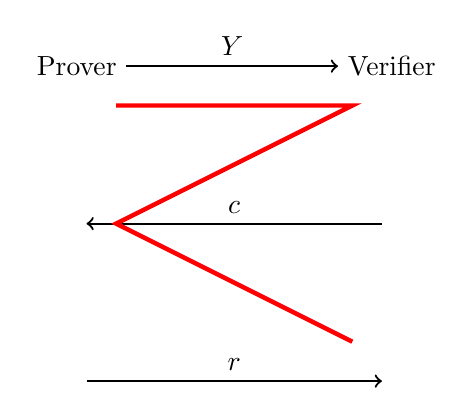
\begin{tikzpicture}
					\node (P1) at (0,0) {Prover};
					\node (V1) at (4,0) {Verifier};
					\node (P2) at (0,-2) {};
					\node (V2) at (4,-2) {};
					\node (P3) at (0,-4) {};
					\node (V3) at (4,-4) {};

					\draw[->, thick] (P1) -- node[above] {$Y$} (V1);
					\draw[->, thick] (V2) -- node[above] {$c$} (P2);
					\draw[->, thick] (P3) -- node[above] {$r$} (V3);

					\draw[red, ultra thick] (0.5,-0.5) -- (3.5,-0.5) -- (0.5,-2) -- (3.5,-3.5);
				\end{tikzpicture}
			\end{center}
		\end{column}
		\begin{column}{0.5\textwidth}
			\textbf{The Greek letter $\Sigma$ (Sigma)}
			\begin{itemize}
				\item Three message flows
				\item Alternating direction
				\item Forms a ``zigzag'' pattern
				\item Hence: Sigma protocols!
			\end{itemize}
			\begin{alertblock}{Always this pattern}
				\begin{enumerate}
					\item Prover $\rightarrow$ Verifier: Commitment
					\item Verifier $\rightarrow$ Prover: Challenge
					\item Prover $\rightarrow$ Verifier: Response
				\end{enumerate}
			\end{alertblock}
		\end{column}
	\end{columns}
\end{frame}

\begin{frame}{Formal definition of Sigma protocols}
	\begin{block}{Definition: Sigma Protocol}
		A sigma protocol consists of the following parameters:
		\begin{itemize}
			\item \textbf{Commit}: A randomized algorithm that takes instance $X$ and witness $W$ as input, outputs commitment $Y$ and state $\sigma$
			\item $\mathcal{C}$: A set of verifier challenges
			\item \textbf{Respond}: A deterministic algorithm that takes state $\sigma$ and challenge $c \in \mathcal{C}$ as input, outputs response $r$
			\item \textbf{Check}: A deterministic algorithm that takes transcript $(X, Y, c, r)$ as input, outputs true/false
		\end{itemize}
	\end{block}
\end{frame}

\begin{frame}{Example: Schnorr as Sigma protocols}
	\begin{columns}[c]
		\begin{column}{0.5\textwidth}
			\textbf{Instance and Witness:}
			\begin{itemize}
				\item Instance: $X = A = g^a$
				\item Witness: $W = a$
				\item Relation: $g^W = X$
			\end{itemize}
			\textbf{The Algorithms:}
			\begin{itemize}
				\item \textbf{Commit}$(A, a)$:
				      \begin{itemize}
					      \item $y \twoheadleftarrow \mathbb{Z}_n$
					      \item $Y = g^y$
					      \item Return $(Y, \sigma = y)$
				      \end{itemize}
			\end{itemize}
		\end{column}
		\begin{column}{0.5\textwidth}
			\begin{itemize}
				\item $\mathcal{C} = \mathbb{Z}_n$ (all possible challenges)
				\item \textbf{Respond}$(\sigma = y, c)$:
				      \begin{itemize}
					      \item Return $r = y + ca \bmod n$
				      \end{itemize}
				\item \textbf{Check}$(A, Y, c, r)$:
				      \begin{itemize}
					      \item Return $(g^r = Y \cdot A^c)$
				      \end{itemize}
			\end{itemize}
			\begin{exampleblock}{Fits the framework!}
				Schnorr is just one example of a Sigma protocol
			\end{exampleblock}
		\end{column}
	\end{columns}
\end{frame}

\begin{frame}{Example: proving knowledge of a representation}
	\begin{columns}[c]
		\begin{column}{0.5\textwidth}
			\textbf{The problem:}
			\begin{itemize}
				\item Given: $X = g^a h^b$
				\item Prove: ``I know $(a, b)$''
				\item Without revealing $(a, b)$!
			\end{itemize}
			\textbf{Why is this useful?}
			\begin{itemize}
				\item Pedersen commitments
				\item Mix networks
				\item Electronic voting
			\end{itemize}
		\end{column}
		\begin{column}{0.5\textwidth}
			\textbf{The Sigma protocol:}
			\begin{itemize}
				\item \textbf{Commit}:
				      \begin{itemize}
					      \item Pick random $r, s$
					      \item $Y = g^r h^s$
					      \item State: $\sigma = (r, s)$
				      \end{itemize}
				\item \textbf{Respond}:
				      \begin{itemize}
					      \item $u = r + ca$
					      \item $v = s + cb$
					      \item Return $(u, v)$
				      \end{itemize}
				\item \textbf{Check}:
				      \begin{itemize}
					      \item $g^u h^v \overset{?}{=} Y \cdot X^c$
				      \end{itemize}
			\end{itemize}
		\end{column}
	\end{columns}
\end{frame}

\begin{frame}{The power of Sigma protocols}
	\begin{center}
		\textbf{Sigma protocols can prove almost any statement!}
	\end{center}
	\vspace{0.5em}
	\begin{columns}[c]
		\begin{column}{0.5\textwidth}
			\textbf{Graph Problems:}
			\begin{itemize}
				\item ``I know a 3-coloring of this graph''
				\item ``I know a Hamiltonian cycle''
				\item ``I know an isomorphism between graphs''
			\end{itemize}
			\textbf{Number Theory:}
			\begin{itemize}
				\item ``I know the square root of $X$ mod $N$''
				\item ``I know the factorization of $N$''
			\end{itemize}
		\end{column}
		\begin{column}{0.5\textwidth}
			\textbf{Cryptographic Statements:}
			\begin{itemize}
				\item ``This ciphertext encrypts 0 or 1''
				\item ``These ciphertexts encrypt the same value''
				\item ``I shuffled these ciphertexts correctly''
			\end{itemize}
			\begin{alertblock}{Universal result}
				Any NP statement has a Sigma protocol!
			\end{alertblock}
		\end{column}
	\end{columns}
\end{frame}

\subsection{Formal Properties of Sigma Protocols}

\begin{frame}{The three essential properties}
	\begin{center}
		\textbf{What makes a Sigma protocol actually work?}
	\end{center}
	\vspace{0.5em}
	\begin{columns}[c]
		\begin{column}{0.5\textwidth}
			\textbf{Mathematical guarantees:}
			\begin{enumerate}
				\item \textbf{Completeness:} Honest provers always succeed
				\item \textbf{Soundness:} Dishonest provers always fail
				\item \textbf{Zero-Knowledge:} Nothing leaks about the witness
			\end{enumerate}
		\end{column}
		\begin{column}{0.5\textwidth}
			\begin{alertblock}{In proof language}
				\begin{itemize}
					\item Completeness: Every true thing has a valid proof
					\item Soundness: Only true things have valid proofs
					\item Zero-Knowledge: Proofs reveal nothing extra
				\end{itemize}
			\end{alertblock}
		\end{column}
	\end{columns}
	\vspace{0.5em}
	\begin{center}
		\textbf{All three are essential for a useful protocol!}
	\end{center}
\end{frame}

\begin{frame}{Completeness: honest provers always win}
	\begin{block}{Definition: Completeness}
		A Sigma protocol is \textbf{complete} if:
		\begin{itemize}
			\item For any instance $X$ and witness $W$ where $P(X,W) = \text{true}$
			\item When the prover follows the protocol honestly
			\item The verifier \textit{always} accepts
		\end{itemize}
	\end{block}
	\vspace{0.5em}
	\textbf{In other words:}
	\begin{itemize}
		\item If you actually know the secret, you can always prove it
		\item No ``false negatives'' - legitimate users never get rejected
		\item The protocol doesn't accidentally lock out honest participants
	\end{itemize}
\end{frame}

\begin{frame}{Example: Schnorr's completeness}
	\begin{center}
		\textbf{Why does Schnorr always work for honest provers?}
	\end{center}
	\vspace{0.5em}
	\begin{columns}[c]
		\begin{column}{0.5\textwidth}
			\textbf{The honest execution:}
			\begin{itemize}
				\item Prover knows $a$ where $A = g^a$
				\item Sends $Y = g^y$ for random $y$
				\item Receives challenge $c$
				\item Responds with $r = y + ca$
			\end{itemize}
		\end{column}
		\begin{column}{0.5\textwidth}
			\textbf{Verification always succeeds:}
			\begin{align*}
				g^r & = g^{y + ca}                   \\
				    & = g^y \cdot g^{ca}             \\
				    & = Y \cdot (g^a)^c              \\
				    & = Y \cdot A^c \quad \checkmark
			\end{align*}
		\end{column}
	\end{columns}
	\vspace{0.5em}
	\begin{exampleblock}{Perfect completeness}
		Honest prover succeeds with probability 1
	\end{exampleblock}
\end{frame}

\begin{frame}{Special soundness: cheaters get caught}{Unique to Sigma protocols}
	\begin{columns}[c]
		\begin{column}{0.6\textwidth}
			\textbf{The challenge for cheaters:}
			\begin{itemize}
				\item Prover doesn't know the witness
				\item Must commit to $Y$ before seeing challenge
				\item Can't predict what challenge will be
				\item Must be ready for \textit{any} challenge!
			\end{itemize}
			\vspace{0.5em}
			\textbf{The extraction principle:}
			\begin{itemize}
				\item If you can answer two different challenges\ldots
				\item \ldots for the same commitment $Y$\ldots
				\item \ldots then you must know the witness!
			\end{itemize}
		\end{column}
		\begin{column}{0.4\textwidth}
			\begin{alertblock}{Key insight}
				Being able to handle multiple challenges proves knowledge
			\end{alertblock}
			\vspace{0.5em}
			\begin{exampleblock}{Why ``special''?}
				This specific form of soundness is unique to Sigma protocols
			\end{exampleblock}
		\end{column}
	\end{columns}
\end{frame}

\begin{frame}{Special soundness: formal definition}
	\begin{block}{Definition: Special Soundness}
		A Sigma protocol has \textbf{special soundness} if there exists an efficient algorithm \textbf{Extract} such that:
		\begin{itemize}
			\item Given two accepting transcripts: $(X, Y, c, r)$ and $(X, Y, c', r')$
			\item With same instance $X$ and commitment $Y$
			\item But different challenges $c \neq c'$
			\item \textbf{Extract}$(X, Y, c, r, c', r')$ outputs witness $W$
			\item Such that $P(X, W) = \text{true}$
		\end{itemize}
	\end{block}
	\vspace{0.5em}
	\textbf{Interpretation:} If you can answer two different challenges for the same commitment, you must know the secret!
\end{frame}

\begin{frame}{Example: extracting from Schnorr}
	\begin{center}
		\textbf{Given two accepting transcripts with same $Y$ but different challenges:}
	\end{center}
	\vspace{0.5em}
	\begin{columns}[c]
		\begin{column}{0.5\textwidth}
			\textbf{Transcript 1:}
			\begin{itemize}
				\item Commitment: $Y$
				\item Challenge: $c$
				\item Response: $r$
				\item Valid: $g^r = Y \cdot A^c$
			\end{itemize}
			\textbf{Transcript 2:}
			\begin{itemize}
				\item Commitment: $Y$ (same!)
				\item Challenge: $c'$
				\item Response: $r'$
				\item Valid: $g^{r'} = Y \cdot A^{c'}$
			\end{itemize}
		\end{column}
		\begin{column}{0.5\textwidth}
			\textbf{Extract the secret:}
			\begin{align*}
				g^r                & = Y \cdot A^c                \\
				g^{r'}             & = Y \cdot A^{c'}             \\
				\frac{g^r}{g^{r'}} & = \frac{A^c}{A^{c'}}         \\
				g^{r-r'}           & = A^{c-c'}                   \\
				g^{r-r'}           & = g^{a(c-c')}                \\
				r-r'               & = a(c-c') \pmod{n}           \\
				a                  & = \frac{r-r'}{c-c'} \pmod{n}
			\end{align*}
		\end{column}
	\end{columns}
\end{frame}

\begin{frame}{Why extraction implies soundness}
	\begin{columns}[c]
		\begin{column}{0.5\textwidth}
			\textbf{The contrapositive argument:}
			\begin{itemize}
				\item If prover doesn't know witness\ldots
				\item Then can't produce two valid responses
				\item So can succeed for at most one challenge
				\item But challenge is random!
				\item Probability of guessing right: $\frac{1}{|\mathcal{C}|}$
			\end{itemize}
		\end{column}
		\begin{column}{0.5\textwidth}
			\begin{alertblock}{Soundness guarantee}
				Cheating probability $\leq \frac{1}{\text{number of challenges}}$
			\end{alertblock}
			\vspace{0.5em}
			\begin{exampleblock}{For Schnorr}
				$|\mathcal{C}| = n$ (prime order)\\
				Cheating probability $\approx \frac{1}{2^{256}}$\\
				Essentially impossible!
			\end{exampleblock}
		\end{column}
	\end{columns}
\end{frame}

\begin{frame}{Zero-knowledge: the formal definition}
	\begin{block}{Definition: Zero-Knowledge}
		A Sigma protocol is \textbf{zero-knowledge} if:
		\begin{itemize}
			\item There exists a simulator algorithm that can generate convincing transcripts
			\item Without knowing the witness!
			\item These simulated transcripts are indistinguishable from real ones
		\end{itemize}
	\end{block}
	\vspace{0.5em}
	\textbf{In other words:}
	\begin{itemize}
		\item If fake transcripts look identical to real ones\ldots
		\item And fake transcripts contain no information about the witness\ldots
		\item Then real transcripts must not leak information either!
		\item We saw this earlier when we proved $\lib{}{schnorr-real} \equiv \lib{}{schnorr-fake}$.
	\end{itemize}
\end{frame}

\begin{frame}{Honest-verifier zero-knowledge}
	\begin{columns}[c]
		\begin{column}{0.5\textwidth}
			\textbf{A subtlety:}
			\begin{itemize}
				\item Sigma protocols are ``honest-verifier'' ZK
				\item Assumes verifier follows the protocol
				\item Chooses challenges randomly
				\item Doesn't try to be clever
			\end{itemize}
			\vspace{0.5em}
			\textbf{What about cheating verifiers?}
			\begin{itemize}
				\item Might choose challenges adaptively
				\item Could try to extract information
				\item Harder to protect against!
			\end{itemize}
		\end{column}
		\begin{column}{0.5\textwidth}
			\begin{exampleblock}{Good news}
				For most applications, honest-verifier ZK is sufficient
			\end{exampleblock}
			\vspace{0.5em}
			\begin{alertblock}{Later: Fiat-Shamir}
				We'll see how to make protocols secure against any verifier by removing interaction entirely!
			\end{alertblock}
		\end{column}
	\end{columns}
\end{frame}

\begin{frame}{Putting it all together}
	\begin{center}
		\textbf{A Sigma protocol is useful when it has all three properties:}
	\end{center}
	\vspace{0.5em}
	\begin{columns}[c]
		\begin{column}{0.33\textwidth}
			\begin{block}{Completeness}
				\begin{itemize}
					\item Honest users succeed
					\item No false rejections
					\item Protocol is usable
				\end{itemize}
			\end{block}
		\end{column}
		\begin{column}{0.33\textwidth}
			\begin{block}{Special Soundness}
				\begin{itemize}
					\item Cheaters get caught
					\item Can extract witness
					\item Protocol is secure
				\end{itemize}
			\end{block}
		\end{column}
		\begin{column}{0.33\textwidth}
			\begin{block}{Zero-Knowledge}
				\begin{itemize}
					\item No information leaks
					\item Privacy preserved
					\item Protocol is private
				\end{itemize}
			\end{block}
		\end{column}
	\end{columns}
	\vspace{1em}
	\begin{center}
		\textbf{Together, these properties create the ``magic'' of zero-knowledge proofs!}
	\end{center}
\end{frame}

\section{Proving AND, OR}

\begin{frame}{Combining proofs: AND and OR}
	\begin{center}
		\textbf{What if we need to prove more complex statements?}
	\end{center}
	\vspace{0.5em}
	\begin{columns}[c]
		\begin{column}{0.5\textwidth}
			\textbf{OR statements:}
			\begin{itemize}
				\item ``I know the private key for $A_1$ OR $A_2$''
				\item ``This vote encrypts YES or NO''
				\item Prove one of several conditions
				\item Without revealing which one!
			\end{itemize}
		\end{column}
		\begin{column}{0.5\textwidth}
			\textbf{AND statements:}
			\begin{itemize}
				\item ``I know $a$ AND $b$ such that\ldots''
				\item ``These discrete logs are equal''
				\item Prove multiple conditions hold
				\item All must be satisfied
			\end{itemize}
		\end{column}
	\end{columns}
	\vspace{0.5em}
	\begin{alertblock}{The challenge}
		How to combine Sigma protocols while preserving zero-knowledge?
	\end{alertblock}
\end{frame}

\subsection{OR Proofs}

\begin{frame}{Example use cases for OR proofs}
	\begin{columns}[c]
		\begin{column}{0.6\textwidth}
			\textbf{1. Anonymous authentication:}
			\begin{itemize}
				\item Public keys: $A_1, A_2$ (authorized users)
				\item Alice proves she knows one private key
				\item Doesn't reveal which user she is!
			\end{itemize}
			\textbf{2. Electronic voting:}
			\begin{itemize}
				\item Encrypted vote: $C = \text{Enc}(\text{vote})$
				\item Prove: $\text{Dec}(SK, C) \in \{\text{yes}, \text{no}\}$
				\item Ensures valid vote without revealing it
			\end{itemize}
		\end{column}
		\begin{column}{0.4\textwidth}
			\begin{exampleblock}{Key property}
				OR proofs hide \textit{which} condition is satisfied
			\end{exampleblock}
			\begin{alertblock}{Privacy guarantee}
				Verifier learns that at least one condition holds, but not which one
			\end{alertblock}
		\end{column}
	\end{columns}
\end{frame}

\begin{frame}{The Robin Hood analogy}
	\begin{columns}[c]
		\begin{column}{0.5\textwidth}
			\begin{itemize}
				\item \textit{Robin Hood has two bows:}
				      \begin{itemize}
					      \item One bow shoots accurately
					      \item One bow is erratic
					      \item King wants proof Robin can shoot well
					      \item But Robin doesn't want to reveal which bow works!
				      \end{itemize}
			\end{itemize}
			\begin{itemize}
				\item \textit{The challenge:}
				      \begin{itemize}
					      \item King draws one target
					      \item Robin must fire both bows
					      \item Arrows must be equidistant from target
				      \end{itemize}
			\end{itemize}
		\end{column}
		\begin{column}{0.5\textwidth}
			\begin{itemize}
				\item \textit{Robin's strategy:}
				      \begin{enumerate}
					      \item Fire the erratic bow first (lands randomly)
					      \item Calculate where to place second arrow
					      \item Use accurate bow to hit that exact spot
					      \item Target appears centered between arrows!
				      \end{enumerate}
				\item \textbf{Control over one arrow is enough to satisfy the constraint}
			\end{itemize}
		\end{column}
	\end{columns}
\end{frame}

\begin{frame}{OR proofs: the construction}
	\textbf{Given:} Sigma protocols $\Sigma_0$ for condition $P_0$ and $\Sigma_1$ for condition $P_1$\\
	\textbf{Goal:} Prove ``I know $W$ such that $P_0(X,W)$ OR $P_1(X,W)$''
	\vspace{0.5em}
	\begin{block}{The protocol}
		\begin{enumerate}
			\item \textbf{Commit:} Prover sends $(Y_0, Y_1)$ - commitments for both protocols
			\item \textbf{Challenge:} Verifier sends single challenge $C$
			\item \textbf{Constraint:} Prover must provide $(C_0, R_0)$ and $(C_1, R_1)$ such that:
			      \begin{itemize}
				      \item $C_0 + C_1 = C$ (challenges sum to verifier's challenge)
				      \item Both transcripts $(Y_0, C_0, R_0)$ and $(Y_1, C_1, R_1)$ are valid
			      \end{itemize}
		\end{enumerate}
	\end{block}
\end{frame}

\begin{frame}{OR proofs: how it works}
	\begin{columns}[c]
		\begin{column}{0.5\textwidth}
			\textbf{If prover knows witness for $P_0$:}
			\begin{enumerate}
				\item Generate real $Y_0$ using witness
				\item Simulate fake transcript for $\Sigma_1$:
				      \begin{itemize}
					      \item Choose random $C_1, R_1$
					      \item Compute $Y_1$ backwards
				      \end{itemize}
				\item Receive challenge $C$ from verifier
				\item Set $C_0 = C - C_1$
				\item Use witness to compute real $R_0$
			\end{enumerate}
		\end{column}
		\begin{column}{0.5\textwidth}
			\textbf{Why it's zero-knowledge:}
			\begin{itemize}
				\item One transcript is real
				\item One transcript is simulated
				\item Verifier can't tell which is which!
				\item Distribution looks identical regardless of which witness we have
			\end{itemize}
			\vspace{0.5em}
			\begin{alertblock}{The trick}
				Prover controls one challenge completely, must adapt to the other
			\end{alertblock}
		\end{column}
	\end{columns}
\end{frame}

\begin{frame}{OR proof protocol diagram}
	\vspace{-1.5cm}
	\begin{center}\resizebox{0.8\textwidth}{!}{
			\begin{msc}{}
				\setmscvalues{small}
				\drawframe{none}
				\setlength{\instdist}{8cm}
				\setlength{\instwidth}{5cm}
				\declinst{prover}{}{Prover (knows $W$ for $P_b$)}
				\declinst{verifier}{}{Verifier}
				\action*{$\begin{array}{l}
							\text{Generate real commitment for } \Sigma_b            \\
							\text{Simulate fake transcript for } \Sigma_{1-b}        \\
							(Y_{1-b}, C_{1-b}, R_{1-b}) \leftarrow \text{Simulate}() \\
						\end{array}$}{prover}
				\nextlevel[5]
				\mess{$(Y_0, Y_1)$}{prover}{verifier}
				\nextlevel[1]
				\action*{$C \twoheadleftarrow \mathcal{C}$}{verifier}
				\nextlevel[2]
				\mess{$C$}{verifier}{prover}
				\nextlevel[1]
				\action*{$\begin{array}{l}
							C_b := C - C_{1-b} \\
							R_b \leftarrow \text{Respond using witness}
						\end{array}$}{prover}
				\nextlevel[4]
				\mess{$(C_0, R_0, C_1, R_1)$}{prover}{verifier}
				\nextlevel[1]
				\action*{$\begin{array}{l}
							\text{Check: } C_0 + C_1 \overset{?}{=} C            \\
							\text{Check: } \Sigma_0.\text{Verify}(Y_0, C_0, R_0) \\
							\text{Check: } \Sigma_1.\text{Verify}(Y_1, C_1, R_1)
						\end{array}$}{verifier}
				\nextlevel[4]
			\end{msc}
		}\end{center}
\end{frame}

\begin{frame}{Example: proving knowledge of one private key}
	\textbf{Setup:} Public keys $A_0 = g^{a_0}$ and $A_1 = g^{a_1}$\\
	\textbf{Alice knows $a_0$ (but not $a_1$) and wants to prove she knows one of them:}
	\begin{enumerate}
		\item \textbf{Commit phase:}
		      \begin{itemize}
			      \item Real: Pick $y_0 \leftarrow \mathbb{Z}_n$, compute $Y_0 = g^{y_0}$
			      \item Fake: Pick $C_1, R_1 \leftarrow \mathbb{Z}_n$, compute $Y_1 = g^{R_1} \cdot A_1^{-C_1}$
			      \item Send $(Y_0, Y_1)$
		      \end{itemize}
		\item \textbf{Challenge:} Receive $C$ from verifier
		\item \textbf{Response phase:}
		      \begin{itemize}
			      \item Compute $C_0 = C - C_1$
			      \item Compute $R_0 = y_0 + C_0 \cdot a_0$
			      \item Send $(C_0, R_0, C_1, R_1)$
		      \end{itemize}
	\end{enumerate}
	\textbf{Verification:} Check $C_0 + C_1 = C$ and both Schnorr transcripts valid
\end{frame}

\subsection{AND Proofs}

\begin{frame}{AND proofs: proving multiple conditions}
	\begin{columns}[c]
		\begin{column}{0.5\textwidth}
			\textbf{The problem:}
			\begin{itemize}
				\item Prove multiple conditions simultaneously
				\item All must be true
				\item Example: ``I know $a$ such that $g_1^a = A_1$ AND $g_2^a = A_2$ AND $g_3^a = A_3$''
			\end{itemize}
			\textbf{Naive approach:}
			\begin{itemize}
				\item Run protocols separately?
				\item Problem: different challenges
				\item Loses zero-knowledge!
			\end{itemize}
		\end{column}
		\begin{column}{0.5\textwidth}
			\textbf{The solution:}
			\begin{itemize}
				\item Use the \textit{same} challenge for all
				\item Commit to all statements
				\item Receive one challenge
				\item Respond to all with same challenge
			\end{itemize}
			\vspace{0.5em}
			\begin{exampleblock}{How it works}
				Reusing the challenge maintains both soundness and zero-knowledge
			\end{exampleblock}
		\end{column}
	\end{columns}
\end{frame}

\begin{frame}{AND proof construction}
	\textbf{Given:} Sigma protocols $\Sigma_1, \Sigma_2, \ldots, \Sigma_k$ for conditions $P_1, P_2, \ldots, P_k$\\
	\textbf{Goal:} Prove ``I know $W$ such that $P_1(X,W)$ AND $P_2(X,W)$ AND \ldots AND $P_k(X,W)$''
	\vspace{0.5em}
	\begin{block}{The protocol}
		\begin{enumerate}
			\item \textbf{Commit:} Run commit phase for all protocols
			      \begin{itemize}
				      \item $(Y_i, \sigma_i) \leftarrow \Sigma_i.\text{Commit}(X_i, W_i)$ for all $i$
				      \item Send $(Y_1, Y_2, \ldots, Y_k)$
			      \end{itemize}
			\item \textbf{Challenge:} Receive single $C$ from verifier
			\item \textbf{Respond:} Use same $C$ for all protocols
			      \begin{itemize}
				      \item $R_i \leftarrow \Sigma_i.\text{Respond}(\sigma_i, C)$ for all $i$
				      \item Send $(R_1, R_2, \ldots, R_k)$
			      \end{itemize}
			\item \textbf{Verify:} Check all transcripts $(Y_i, C, R_i)$ are valid
		\end{enumerate}
	\end{block}
\end{frame}

\begin{frame}{Example: proving equality of discrete logs}
	\textbf{Setup:} Given $(g_1, g_2, g_3, A_1, A_2, A_3)$ where $A_i = g_i^a$ for same $a$\\
	\textbf{Protocol to prove knowledge of $a$:}
	\begin{columns}[c]
		\begin{column}{0.5\textwidth}
			\begin{enumerate}
				\item \textbf{Commit:}
				      \begin{itemize}
					      \item Pick $y \leftarrow \mathbb{Z}_n$
					      \item Compute $Y_1 = g_1^y$
					      \item Compute $Y_2 = g_2^y$
					      \item Compute $Y_3 = g_3^y$
					      \item Send $(Y_1, Y_2, Y_3)$
				      \end{itemize}
				\item \textbf{Challenge:} Receive $C$
			\end{enumerate}
		\end{column}
		\begin{column}{0.5\textwidth}
			\begin{enumerate}
				\setcounter{enumi}{2}
				\item \textbf{Respond:}
				      \begin{itemize}
					      \item Compute $R = y + C \cdot a$
					      \item Send $R$
				      \end{itemize}
				\item \textbf{Verify:}
				      \begin{itemize}
					      \item Check $g_1^R = Y_1 \cdot A_1^C$
					      \item Check $g_2^R = Y_2 \cdot A_2^C$
					      \item Check $g_3^R = Y_3 \cdot A_3^C$
				      \end{itemize}
			\end{enumerate}
		\end{column}
	\end{columns}
	\vspace{0.5em}
	\begin{alertblock}{Single response proves all!}
		One value $R$ satisfies all three equations if and only if all discrete logs are equal
	\end{alertblock}
\end{frame}

\begin{frame}{Combining AND and OR}
	\begin{center}
		\textbf{We can build complex logical statements!}
	\end{center}
	\vspace{0.5em}
	\textbf{Example:} ``I know the private key for ($A_1$ OR $A_2$) AND ($B_1$ OR $B_2$)''
	\begin{itemize}
		\item Meaning: I'm one of users $\{A_1, A_2\}$ AND one of users $\{B_1, B_2\}$
		\item Four possible combinations, but verifier learns nothing about which!
	\end{itemize}
	\vspace{0.5em}
	\textbf{Construction approach:}
	\begin{enumerate}
		\item Build OR protocols for each clause
		\item Combine them using AND construction
		\item Result: Single protocol proving the entire statement
	\end{enumerate}
\end{frame}

\section{Non-Interactive Zero-Knowledge Proofs}

\subsection{Fiat-Shamir}

\begin{frame}{Non-interactive proofs: removing the verifier}
	\begin{center}
		\textbf{The limitation of interactive proofs}
	\end{center}
	\vspace{0.5em}
	\begin{columns}[c]
		\begin{column}{0.5\textwidth}
			\textbf{Interactive Sigma protocols:}
			\begin{itemize}
				\item Require back-and-forth communication
				\item Prover and verifier must be online together
				\item Can't post a proof for later verification
				\item Can't broadcast a proof to many verifiers
			\end{itemize}
		\end{column}
		\begin{column}{0.5\textwidth}
			\textbf{What we want:}
			\begin{itemize}
				\item Prover generates proof alone
				\item Anyone can verify later
				\item No interaction needed
				\item But still zero-knowledge!
			\end{itemize}
			\vspace{0.5em}
			\begin{alertblock}{The challenge}
				How to ensure $C$ comes after $Y$ without a verifier?
			\end{alertblock}
		\end{column}
	\end{columns}
\end{frame}

\begin{frame}{The Fiat-Shamir transformation}
	\begin{center}
		\textbf{Replace the verifier with a hash function!}
	\end{center}
	\vspace{0.5em}
	\begin{columns}[c]
		\begin{column}{0.5\textwidth}
			\begin{itemize}
				\item \textbf{Requirements:}
				      \begin{itemize}
					      \item Challenge must be unpredictable
					      \item Must depend on commitment $Y$
					      \item Solution: $C := \func{hash}{X, Y}$
					      \item Hash function acts as ``virtual verifier''
				      \end{itemize}
			\end{itemize}
			\begin{itemize}
				\item \textbf{Properties needed:}
				      \begin{itemize}
					      \item $H$ modeled as random oracle
					      \item Output unpredictable before input
					      \item Uniformly distributed output
				      \end{itemize}
			\end{itemize}
		\end{column}
		\begin{column}{0.5\textwidth}
			\begin{exampleblock}{Random oracle}
				\begin{itemize}
					\item A theoretical hash function that:
					      \begin{itemize}
						      \item Returns random output for each new input
						      \item Always returns same output for same input
						      \item Output is uniformly distributed
					      \end{itemize}
					\item In practice, we use SHA-256 or similar, which approximates these properties
				\end{itemize}
			\end{exampleblock}
		\end{column}
	\end{columns}
\end{frame}

\begin{frame}{Fiat-Shamir: the construction}
	Given a Sigma protocol $\Sigma$, create a non-interactive proof system:\\[1em]
	\begin{columns}[c]
		\begin{column}{0.5\textwidth}
			\textbf{Prove}$(X, W)$:
			\begin{enumerate}
				\item $(Y, \sigma) := \Sigma.\text{Commit}(X, W)$
				\item \hl{$C := \func{hash}{X, Y}$}
				\item $R := \Sigma.\text{Respond}(\sigma, C)$
				\item Return $(Y, R)$
			\end{enumerate}
		\end{column}
		\begin{column}{0.5\textwidth}
			\textbf{Verify}$(X, Y, R)$:
			\begin{enumerate}
				\item \hl{$C := \func{hash}{X, Y}$}
				\item Return $\Sigma.\text{Check}(X, Y, C, R)$
			\end{enumerate}
		\end{column}
	\end{columns}
	\vspace{0.5em}
	\begin{center}
		\textbf{The proof is just $(Y, R)$ - no interaction needed!}
	\end{center}
\end{frame}

\begin{frame}{Example: Non-interactive Schnorr}
	\begin{columns}[c]
		\begin{column}{0.5\textwidth}
			\textbf{Interactive Schnorr:}
			\begin{enumerate}
				\item Prover sends $Y = g^y$
				\item Verifier sends random $c$
				\item Prover sends $r = y + ca$
				\item Verifier checks $g^r = Y \cdot A^c$
			\end{enumerate}
		\end{column}
		\begin{column}{0.5\textwidth}
			\textbf{Fiat-Shamir Schnorr:}
			\begin{enumerate}
				\item Prover computes $Y = g^y$
				\item Prover computes $c = \func{hash}{A, Y}$
				\item Prover computes $r = y + ca$
				\item Proof is $(Y, r)$
				\item Verifier recomputes $c = \func{hash}{A, Y}$
				\item Verifier checks $g^r = Y \cdot A^c$
			\end{enumerate}
		\end{column}
	\end{columns}
	\vspace{0.5em}
	\begin{alertblock}{This is a digital signature!}
		If we include a message $m$ in the hash: $c = \func{hash}{A, Y, m}$, we get the Schnorr signature scheme!
	\end{alertblock}
\end{frame}

\begin{frame}{Why Fiat-Shamir is sound}
	\begin{center}
		\textbf{The order of operations is crucial}
	\end{center}
	\begin{columns}[c]
		\begin{column}{0.5\textwidth}
			\begin{itemize}
				\item \textbf{With random oracle:}
				      \begin{itemize}
					      \item Must choose $Y$ first
					      \item Then compute $C = \func{hash}{X, Y}$
					      \item Can't predict $C$ before choosing $Y$
					      \item Can't ``work backwards'' like in simulation
				      \end{itemize}
			\end{itemize}
			\begin{itemize}
				\item \textbf{This enforces honest behavior:}
				      \begin{itemize}
					      \item Prover commits before seeing challenge
					      \item Just like in interactive protocol
					      \item Hash function enforces ordering
				      \end{itemize}
			\end{itemize}
		\end{column}
		\begin{column}{0.5\textwidth}
			\begin{alertblock}{Key difference from interactive}
				\begin{itemize}
					\item In interactive Sigma protocol:
					      \begin{itemize}
						      \item Can simulate by choosing $C, R$ first
						      \item Then compute $Y$ backwards
						      \item This creates deniability
					      \end{itemize}
				\end{itemize}
				\begin{itemize}
					\item In Fiat-Shamir:
					      \begin{itemize}
						      \item Can't choose $C$ arbitrarily
						      \item Must be $C = \func{hash}{X, Y}$
						      \item Can't work backwards!
						      \item \textbf{Loses deniability property}
					      \end{itemize}
				\end{itemize}
			\end{alertblock}
		\end{column}
	\end{columns}
\end{frame}

\begin{frame}{The Forking Lemma: extracting witnesses}
	\begin{block}{Lemma (Forking Lemma)}
		If an algorithm $A$ can produce valid Fiat-Shamir proofs with non-negligible probability, then we can extract a valid witness with non-negligible probability.
	\end{block}
	\vspace{0.5em}
	\textbf{The extraction strategy:}
	\begin{enumerate}
		\item Run $A$ until it outputs valid proof $(Y, R)$
		\item ``Rewind'' $A$ to when it queried $\func{hash}{X, Y}$
		\item Give a different hash output $C'$ this time
		\item If $A$ outputs another valid proof with same $Y$:
		      \begin{itemize}
			      \item We have two transcripts: $(Y, C, R)$ and $(Y, C', R')$
			      \item Extract witness using special soundness!
		      \end{itemize}
	\end{enumerate}
\end{frame}

\begin{frame}{Forking Lemma: the challenge}
	\begin{columns}[c]
		\begin{column}{0.5\textwidth}
			\textbf{Why extraction is tricky:}
			\begin{itemize}
				\item $A$ might query hash many times
				\item Don't know which query to rewind to
				\item After rewinding, $A$ might:
				      \begin{itemize}
					      \item Not output a valid proof
					      \item Output proof with different $Y$
					      \item Behave completely differently
				      \end{itemize}
			\end{itemize}
		\end{column}
		\begin{column}{0.5\textwidth}
			\textbf{The solution:}
			\begin{itemize}
				\item Save state at every hash query
				\item After valid proof, rewind to $\func{hash}{X, Y}$
				\item Try multiple times if needed
				\item Analysis shows this works with non-negligible probability
			\end{itemize}
		\end{column}
	\end{columns}
\end{frame}

\begin{frame}{Deniability lost!}
	\begin{center}
		\textbf{Fiat-Shamir destroys the deniability property}
	\end{center}
	\vspace{0.5em}
	\begin{columns}[c]
		\begin{column}{0.5\textwidth}
			\textbf{Interactive Sigma protocol:}
			\begin{itemize}
				\item Transcripts are deniable
				\item Anyone can generate fake transcripts
				\item Choose $C, R$ first, compute $Y$
				\item Indistinguishable from real
				\item \textbf{Can't prove to third parties}
			\end{itemize}
		\end{column}
		\begin{column}{0.5\textwidth}
			\textbf{Fiat-Shamir proof:}
			\begin{itemize}
				\item Have constraint $C = \func{hash}{X, Y}$
				\item Everyone can verify this constraint
				\item Can't generate fake proofs
				\item Only witness holder can create
				\item \textbf{Transferable evidence!}
			\end{itemize}
		\end{column}
	\end{columns}
	\vspace{0.5em}
	\begin{alertblock}{Trade-off}
		We gain non-interactivity but lose deniability. The proof becomes a permanent, transferable piece of evidence.
	\end{alertblock}
\end{frame}

\begin{frame}{Applications of Fiat-Shamir}
	\begin{center}
		\textbf{Fiat-Shamir is widely used in practice}
	\end{center}
	\vspace{0.5em}
	\begin{columns}[c]
		\begin{column}{0.5\textwidth}
			\textbf{Digital signatures:}
			\begin{itemize}
				\item Schnorr signatures
				\item EdDSA (used in many systems)
				\item BLS signatures (with pairings)
			\end{itemize}
			\vspace{0.5em}
			\textbf{Blockchain applications:}
			\begin{itemize}
				\item Proof of reserves
				\item Ring signatures for privacy
				\item Bulletproofs (range proofs)
			\end{itemize}
		\end{column}
		\begin{column}{0.5\textwidth}
			\textbf{Advanced protocols:}
			\begin{itemize}
				\item SNARKs (succinct proofs)
				\item STARKs (transparent proofs)
				\item Proof of knowledge of signature
			\end{itemize}
			\vspace{0.5em}
			\begin{alertblock}{Key advantage}
				Convert any interactive ZK proof into a non-interactive one that can be verified by anyone, anytime
			\end{alertblock}
		\end{column}
	\end{columns}
\end{frame}

\subsection{Fiat-Shamir Circuits}

\begin{frame}{From statements to circuits: a paradigm shift}
	\begin{center}
		\textbf{Wait, why are we suddenly talking about circuits?}
	\end{center}
	\vspace{0.5em}
	\begin{columns}[c]
		\begin{column}{0.5\textwidth}
			\textbf{So far, we proved statements like:}
			\begin{itemize}
				\item ``I know $a$ such that $g^a = A$''
				\item ``I know a 3-coloring of this graph''
				\item Specific mathematical relations
			\end{itemize}
			\vspace{0.5em}
			\textbf{But what if we want to prove:}
			\begin{itemize}
				\item ``I computed this SHA-256 correctly''
				\item ``This transaction is valid''
				\item ``I executed this program correctly''
			\end{itemize}
		\end{column}
		\begin{column}{0.5\textwidth}
			\begin{alertblock}{The idea}
				Any computation can be represented as a circuit!
			\end{alertblock}
			\vspace{0.5em}
			\begin{exampleblock}{Think of it like:}
				Instead of proving ``I know $x$'', we prove ``I know $x$ such that circuit $C(x) = y$''
			\end{exampleblock}
		\end{column}
	\end{columns}
\end{frame}

\begin{frame}{What is a circuit?}
	\begin{columns}[c]
		\begin{column}{0.5\textwidth}
			\begin{itemize}
				\item \textbf{A circuit is just a computation graph:}
				      \begin{itemize}
					      \item Gates: AND, OR, NOT, ADD, MUL, etc.
					      \item Wires: Connect gates together
					      \item Inputs: Public ($x$) and private ($w$)
					      \item Output: Result of computation
				      \end{itemize}
				\item \textbf{Example: $y = (a + b) \cdot c$}
				      \begin{center}
					      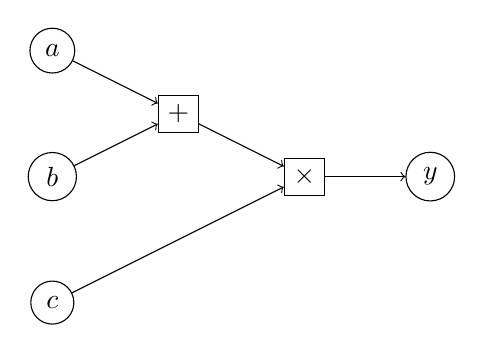
\begin{tikzpicture}[scale=0.8]
						      \node[circle,draw] (a) at (0,2) {$a$};
						      \node[circle,draw] (b) at (0,0) {$b$};
						      \node[circle,draw] (c) at (0,-2) {$c$};
						      \node[rectangle,draw] (add) at (2,1) {$+$};
						      \node[rectangle,draw] (mul) at (4,0) {$\times$};
						      \node[circle,draw] (y) at (6,0) {$y$};

						      \draw[->] (a) -- (add);
						      \draw[->] (b) -- (add);
						      \draw[->] (add) -- (mul);
						      \draw[->] (c) -- (mul);
						      \draw[->] (mul) -- (y);
					      \end{tikzpicture}
				      \end{center}
			\end{itemize}
		\end{column}
		\begin{column}{0.5\textwidth}
			\begin{itemize}
				\item \textbf{Why circuits?}
				      \begin{itemize}
					      \item Universal representation
					      \item Any algorithm $\rightarrow$ circuit
					      \item Fixed structure (no loops!)
					      \item Easy to verify gate-by-gate
				      \end{itemize}
			\end{itemize}
			\begin{exampleblock}{The power}
				Once we can prove statements about circuits, we can prove statements about \textit{any computation}!
			\end{exampleblock}
		\end{column}
	\end{columns}
\end{frame}

\begin{frame}{The zero-knowledge circuit paradigm}
	\begin{center}
		\textbf{The fundamental shift in thinking}
	\end{center}
	\vspace{0.5em}
	\begin{columns}[c]
		\begin{column}{0.5\textwidth}
			\textbf{Old way (Sigma protocols):}
			\begin{itemize}
				\item Design specific protocol for each statement
				\item Schnorr for discrete log
				\item Different protocol for factoring
				\item Custom protocol for each problem
			\end{itemize}
		\end{column}
		\begin{column}{0.5\textwidth}
			\textbf{New way (Circuit ZK):}
			\begin{itemize}
				\item Convert problem to circuit
				\item Use general ZK protocol for circuits
				\item Same protocol works for everything!
				\item Just change the circuit
			\end{itemize}
		\end{column}
	\end{columns}
	\vspace{0.5em}
	\begin{alertblock}{This changes everything!}
		Instead of crafting clever protocols, we write programs and prove we executed them correctly
	\end{alertblock}
\end{frame}

\begin{frame}{Example: proving knowledge of a hash preimage}
	\begin{center}
		\textbf{Claim: ``I know $x$ such that SHA256($x$) = $y$''}
	\end{center}
	\vspace{0.5em}
	\begin{columns}[c]
		\begin{column}{0.5\textwidth}
			\textbf{As a Sigma protocol:}
			\begin{itemize}
				\item Would be incredibly complex
				\item SHA-256 has 64 rounds
				\item Each round has bitwise operations
				\item No elegant mathematical structure
				\item Basically impossible to design!
			\end{itemize}
		\end{column}
		\begin{column}{0.5\textwidth}
			\textbf{As a circuit:}
			\begin{itemize}
				\item Write SHA-256 as circuit
				\item Input: private $x$
				\item Output: public $y$
				\item Apply general circuit ZK protocol
				\item Done! Works automatically
			\end{itemize}
		\end{column}
	\end{columns}
\end{frame}

\begin{frame}[fragile]{From theory to practice: ZK programming}
	\begin{columns}[c]
		\begin{column}{0.5\textwidth}
			\textbf{Modern ZK development:}
			\begin{itemize}
				\item Write programs in high-level languages
				\item Compiler converts to circuits
				\item ZK protocol proves circuit execution
				\item Developer doesn't see the circuit!
			\end{itemize}
			\vspace{0.5em}
			\textbf{Example (Circom syntax):}
			\begin{verbatim}
template IsZero() {
  signal input in;
  signal output out;
  // Proves: out = (in == 0)
}
   \end{verbatim}
		\end{column}
		\begin{column}{0.5\textwidth}
			\textbf{The compilation pipeline:}
			\begin{enumerate}
				\item High-level code
				\item Intermediate representation
				\item Arithmetic circuit
				\item Constraint system
				\item ZK proof
			\end{enumerate}
			\vspace{0.5em}
			\begin{alertblock}{We've come full circle}
				Started with ``I know a secret''\\
				Now: ``I ran this program correctly''\\
				Both use the same ZK machinery!
			\end{alertblock}
		\end{column}
	\end{columns}
\end{frame}

\begin{frame}{The cost of generality}
	\begin{center}
		\textbf{Circuit ZK is powerful but comes with trade-offs}
	\end{center}
	\vspace{0.5em}
	\begin{columns}[c]
		\begin{column}{0.5\textwidth}
			\textbf{Advantages:}
			\begin{itemize}
				\item Universal - works for any computation
				\item Compositional - combine circuits
				\item Tool support - compilers, libraries
				\item No need for crypto expertise
			\end{itemize}
		\end{column}
		\begin{column}{0.5\textwidth}
			\textbf{Disadvantages:}
			\begin{itemize}
				\item Less efficient than custom protocols
				\item Circuit can be huge (millions of gates)
				\item Proving time can be slow
				\item More complex security analysis
			\end{itemize}
		\end{column}
	\end{columns}
	\vspace{0.5em}
	\begin{exampleblock}{Rule of thumb}
		Use custom Sigma protocols for simple statements (like Schnorr)\\
		Use circuit ZK for complex computations (like program execution)
	\end{exampleblock}
\end{frame}

\subsection{Attacks on Fiat-Shamir}

\begin{frame}{The problem with Fiat-Shamir}
	\begin{center}
		\textbf{Can we actually trust Fiat-Shamir in practice?}
	\end{center}
	\vspace{0.5em}
	\begin{columns}[c]
		\begin{column}{0.5\textwidth}
			\textbf{The promise:}
			\begin{itemize}
				\item FS is secure in random oracle model
				\item Replace oracle with concrete hash
				\item Should be secure in practice
			\end{itemize}
			\vspace{0.5em}
			\textbf{Known theoretical attacks:}
			\begin{itemize}
				\item Canetti-Goldreich-Halevi (2004)
				\item Barak (2001), Goldwasser-Kalai (2003)
				\item But all use contrived protocols!
			\end{itemize}
		\end{column}
		\begin{column}{0.5\textwidth}
			\begin{alertblock}{New result (2025)}
				First practical attack on a standard protocol!\footnote{https://appliedcryptography.page/papers/\#prove-false}
				\begin{itemize}
					\item Targets GKR-based proof systems
					\item Used in real deployed systems
					\item Attack works for \textit{any} hash function
				\end{itemize}
			\end{alertblock}
		\end{column}
	\end{columns}
\end{frame}

\begin{frame}{The GKR protocol under attack}
	\begin{columns}[c]
		\begin{column}{0.5\textwidth}
			\textbf{What is GKR?}
			\begin{itemize}
				\item Protocol by Goldwasser-Kalai-Rothblum
				\item Proves correctness of computations
				\item Works for bounded-depth circuits
				\item Combined with polynomial commitments
			\end{itemize}
			\vspace{0.5em}
			\textbf{The claim being proved:}
			\begin{itemize}
				\item Circuit $C$, input $x$, witness $w$
				\item Prove: $\exists w$ such that $C(x,w) = y$
			\end{itemize}
		\end{column}
		\begin{column}{0.5\textwidth}
			\textbf{Why this matters:}
			\begin{itemize}
				\item Widely studied in literature
				\item Used in practice (e.g., Expander)
				\item Considered secure with Fiat-Shamir
				\item Foundation of many SNARKs
			\end{itemize}
			\vspace{0.5em}
			\begin{exampleblock}{The protocol flow}
				\begin{enumerate}
					\item Commit to witness $w$
					\item Verifier picks random $r$
					\item Run GKR reduction
					\item Verify with polynomial commitment
				\end{enumerate}
			\end{exampleblock}
		\end{column}
	\end{columns}
\end{frame}

\begin{frame}{Extended attack: backdooring any circuit}
	\begin{center}
		\textbf{We can insert a backdoor into ANY circuit!}
	\end{center}
	\vspace{0.5em}
	\begin{columns}[c]
		\begin{column}{0.5\textwidth}
			\textbf{Given:}
			\begin{itemize}
				\item Any circuit $C(x,w) \rightarrow y$
				\item Desired input $x^*$ and output $y^*$
			\end{itemize}
			\vspace{0.5em}
			\textbf{We construct:}
			\begin{itemize}
				\item Circuit $C^*$ functionally equivalent to $C$
				\item But can prove $C^*(x^*, w) = y^*$
				\item Even if this is FALSE!
			\end{itemize}
		\end{column}
		\begin{column}{0.5\textwidth}
			\textbf{The backdoored circuit:}
			\begin{enumerate}
				\item Compute $y = C(x,w)$ normally
				\item Check if conditions match attack
				\item If yes, manipulate output
				\item Otherwise, output $y$
			\end{enumerate}
			\vspace{0.5em}
			\begin{alertblock}{Critical insight}
				Security depends on circuit \textit{implementation}, not just functionality!
			\end{alertblock}
		\end{column}
	\end{columns}
\end{frame}

\begin{frame}{Implications for practice}
	\begin{center}
		\textbf{What does this mean for real systems?}
	\end{center}
	\vspace{0.5em}
	\begin{columns}[c]
		\begin{column}{0.5\textwidth}
			\textbf{Immediate impact:}
			\begin{itemize}
				\item GKR+FS is not secure in general
				\item Affects deployed systems
				\item No ``safe'' hash function choice
				\item Circuit implementation matters!
			\end{itemize}
			\vspace{0.5em}
			\textbf{Particularly concerning:}
			\begin{itemize}
				\item Recursive proof composition
				\item Circuits that use crypto primitives
				\item Hard to audit implementations
			\end{itemize}
		\end{column}
		\begin{column}{0.5\textwidth}
			\textbf{Mitigations:}
			\begin{itemize}
				\item Restrict circuit depth
				\item Avoid circuits with crypto ops
				\item Use canonical representations
				\item Domain separation techniques
			\end{itemize}
			\vspace{0.5em}
			\begin{exampleblock}{Silver lining}
				Simple circuits (e.g., for lookups) seem safe - they have canonical forms
			\end{exampleblock}
		\end{column}
	\end{columns}
\end{frame}

\begin{frame}{Lessons learned}
	\begin{center}
		\textbf{The Fiat-Shamir transform is more fragile than we thought}
	\end{center}
	\vspace{0.5em}
	\begin{columns}[c]
		\begin{column}{0.5\textwidth}
			\textbf{Key takeaways:}
			\begin{itemize}
				\item Random oracle model $\neq$ real world
				\item Natural protocols can fail
				\item Implementation details matter
				\item Need extreme care in practice
			\end{itemize}
			\vspace{0.5em}
			\textbf{Open questions:}
			\begin{itemize}
				\item Which protocols are safe?
				\item Better security models?
				\item Practical alternatives to FS?
			\end{itemize}
		\end{column}
		\begin{column}{0.5\textwidth}
			\begin{alertblock}{Remember}
				\begin{itemize}
					\item This isn't a hash function weakness
					\item It's a fundamental protocol issue
					\item Affects any FS hash choice
					\item First attack on ``real'' protocol
				\end{itemize}
			\end{alertblock}
			\vspace{0.5em}
			\begin{exampleblock}{Future work}
				Need provably secure alternatives based on standard assumptions
			\end{exampleblock}
		\end{column}
	\end{columns}
\end{frame}

\section{Zero-Knowledge Proofs in the Real World}

\subsection{Zcash: Privacy-Preserving Cryptocurrency}

\begin{frame}{Zcash: bringing ZK to cryptocurrency}
	\begin{columns}[c]
		\begin{column}{0.5\textwidth}
			\begin{itemize}
				\item \textbf{Bitcoin's transparency:}
				      \begin{itemize}
					      \item All transactions are public
					      \item Addresses are pseudonymous
					      \item But can be linked and traced
					      \item Chain analysis reveals patterns
					      \item Privacy through obscurity fails
				      \end{itemize}
				\item \textbf{The need for privacy:}
				      \begin{itemize}
					      \item Financial privacy is fundamental
					      \item Fungibility requires privacy
					      \item Businesses need confidentiality
				      \end{itemize}
			\end{itemize}
		\end{column}
		\begin{column}{0.5\textwidth}
			\begin{itemize}
				\item \textbf{Enter Zcash (2016):}
				      \begin{itemize}
					      \item First production use of zk-SNARKs
					      \item Optional privacy for transactions
					      \item Prove transaction validity without revealing:
					            \begin{itemize}
						            \item Sender
						            \item Receiver
						            \item Amount
					            \end{itemize}
					      \item Revolutionary achievement!
				      \end{itemize}
			\end{itemize}
		\end{column}
	\end{columns}
\end{frame}

\begin{frame}{How Zcash works: shielded transactions}
	\begin{columns}[c]
		\begin{column}{0.5\textwidth}
			\textbf{Two types of addresses:}
			\begin{itemize}
				\item \textbf{Transparent (t-addresses):}
				      \begin{itemize}
					      \item Work like Bitcoin
					      \item Fully visible on blockchain
					      \item Start with 't'
				      \end{itemize}
				\item \textbf{Shielded (z-addresses):}
				      \begin{itemize}
					      \item Use zero-knowledge proofs
					      \item Hide transaction details
					      \item Start with 'z'
				      \end{itemize}
			\end{itemize}
		\end{column}
		\begin{column}{0.5\textwidth}
			\textbf{What the ZK proof proves:}
			\begin{itemize}
				\item Input notes exist
				\item Sender owns the input notes
				\item No double spending
			\end{itemize}
			\vspace{0.5em}
			\begin{alertblock}{The magic}
				All this is proved without revealing which notes are spent or created!
			\end{alertblock}
		\end{column}
	\end{columns}
\end{frame}

\begin{frame}{Evolution and improvements}
	\begin{columns}[c]
		\begin{column}{0.5\textwidth}
			\textbf{Performance journey:}
			\begin{itemize}
				\item \textbf{Sprout (2016):}
				      \begin{itemize}
					      \item Proof generation: ~40 seconds
					      \item Memory: ~3 GB
					      \item Mobile impossible
				      \end{itemize}
				\item \textbf{Sapling (2018):}
				      \begin{itemize}
					      \item Proof generation: ~2.5 seconds
					      \item Memory: ~40 MB
					      \item Mobile feasible
				      \end{itemize}
				\item \textbf{Halo 2 (Today):}
				      \begin{itemize}
					      \item No trusted setup!
					      \item Recursive proofs
					      \item Even better performance
				      \end{itemize}
			\end{itemize}
		\end{column}
		\begin{column}{0.5\textwidth}
			\textbf{Key innovations:}
			\begin{itemize}
				\item Viewing keys for auditing
				\item Memo field for encrypted messages
				\item Unified addresses
				\item Hardware wallet support
			\end{itemize}
			\vspace{0.5em}
			\begin{alertblock}{The trade-off}
				Privacy comes at a cost: shielded transactions are more expensive and complex than transparent ones
			\end{alertblock}
		\end{column}
	\end{columns}
\end{frame}

\begin{frame}{Impact and lessons learned}
	\begin{columns}[c]
		\begin{column}{0.5\textwidth}
			\textbf{Technical achievements:}
			\begin{itemize}
				\item First production ZK system at scale
				\item Proved ZK can work in adversarial environment
				\item Inspired countless other projects
				\item Advanced the field significantly
			\end{itemize}
			\vspace{0.5em}
			\textbf{Challenges faced:}
			\begin{itemize}
				\item Regulatory concerns
				\item Exchange delistings
				\item Slow progress and growth
			\end{itemize}
		\end{column}
		\begin{column}{0.5\textwidth}
			\textbf{Lessons for ZK adoption:}
			\begin{itemize}
				\item Privacy must be easy to use
				\item Optional privacy \rightarrow\ limited adoption
				\item Performance matters enormously
				\item Trust assumptions are critical
				\item Regulatory environment is key
			\end{itemize}
			\vspace{0.5em}
			\begin{exampleblock}{Legacy}
				Zcash showed the world that zero-knowledge proofs aren't just theory - they can secure billions in value
			\end{exampleblock}
		\end{column}
	\end{columns}
\end{frame}

\subsection{ZK Goes Mainstream: Google's Open Source Initiative}

\begin{frame}{From academic curiosity to industry adoption}
	\begin{columns}[c]
		\begin{column}{0.5\textwidth}
			\textbf{What just happened?}
			\begin{itemize}
				\item Google open-sourced ZKP libraries
				\item Partnership with Sparkasse (German bank)
				\item Focus on EU age assurance
				\item Code available on GitHub\footnote{https://github.com/google/longfellow-zk}
			\end{itemize}
			\vspace{0.5em}
			\textbf{Why this matters:}
			\begin{itemize}
				\item Tech giant embracing privacy tech
				\item Real-world deployment at scale
				\item Not just research anymore!
			\end{itemize}
		\end{column}
		\begin{column}{0.5\textwidth}
			\begin{exampleblock}{The promise fulfilled}
				``In layperson's terms, ZKP makes it possible for people to prove that something about them is true without exchanging any other data.''
			\end{exampleblock}
			\vspace{0.5em}
			\begin{alertblock}{Think about it}
				We've spent this lecture learning the theory. Now it's becoming everyday technology!
			\end{alertblock}
		\end{column}
	\end{columns}
\end{frame}

\begin{frame}{The age verification problem}
	\begin{columns}[c]
		\begin{column}{0.5\textwidth}
			\textbf{Current approaches:}
			\begin{itemize}
				\item Upload government ID
				\item Credit card verification
				\item Face recognition + AI
				\item Third-party identity services
			\end{itemize}
			\vspace{0.5em}
			\textbf{Problems:}
			\begin{itemize}
				\item Privacy nightmare
				\item Data breaches
				\item Identity theft risk
				\item Tracking across sites
			\end{itemize}
		\end{column}
		\begin{column}{0.5\textwidth}
			\textbf{The ZK solution:}
			\begin{itemize}
				\item Prove: ``I am over 18''
				\item Reveal: Nothing else!
				\item No name, no birthdate
				\item No tracking possible
				\item Cryptographically secure
			\end{itemize}
			\vspace{0.5em}
			\begin{block}{Question for you}
				What other attributes could we prove this way? Think beyond age...
			\end{block}
		\end{column}
	\end{columns}
\end{frame}

\begin{frame}{The European regulatory landscape}
	\begin{columns}[c]
		\begin{column}{0.5\textwidth}
			\textbf{eIDAS Regulation (2026):}
			\begin{itemize}
				\item European Digital Identity Wallet
				\item Every EU citizen gets one
				\item Must work across all member states
				\item Privacy-enhancing tech encouraged
			\end{itemize}
			\textbf{The tension:}
			\begin{itemize}
				\item Governments want: Control, compliance
				\item Citizens want: Privacy, freedom
				\item ZK offers: Both! Or does it?
			\end{itemize}
		\end{column}
		\begin{column}{0.5\textwidth}
			\begin{alertblock}{Critical thinking}
				\begin{itemize}
					\item Is this true privacy protection?
					\item Who controls the infrastructure?
					\item Can governments revoke proofs?
					\item What about metadata leakage?
				\end{itemize}
			\end{alertblock}
			\begin{exampleblock}{Looking for extra credit?}
				Research the EUDI Wallet proposal. Does it truly protect privacy or just shift trust?
			\end{exampleblock}
		\end{column}
	\end{columns}
\end{frame}

\begin{frame}{The open source angle: democratizing privacy}
	\begin{columns}[c]
		\begin{column}{0.5\textwidth}
			\textbf{Benefits of open sourcing:}
			\begin{itemize}
				\item Transparency - no backdoors
				\item Community review
				\item Faster innovation
				\item No vendor lock-in
				\item Educational value
			\end{itemize}
			\textbf{The ecosystem effect:}
			\begin{itemize}
				\item Developers can build on it
				\item Researchers can improve it
				\item Standards can emerge
			\end{itemize}
		\end{column}
		\begin{column}{0.5\textwidth}
			\textbf{But consider:}
			\begin{itemize}
				\item Google's motivations?
				\item Control through contribution?
				\item Patent considerations?
				\item Implementation vs. specification
			\end{itemize}
		\end{column}
	\end{columns}
\end{frame}

\begin{frame}{Beyond age verification: the possibilities}
	\begin{center}
		\textbf{Where else could ZK proofs transform our digital lives?}
	\end{center}
	\vspace{0.5em}
	\begin{columns}[c]
		\begin{column}{0.5\textwidth}
			\textbf{Financial services:}
			\begin{itemize}
				\item Prove income without revealing amount
				\item Credit worthiness without credit score
				\item KYC without identity exposure
			\end{itemize}
			\vspace{0.5em}
			\textbf{Healthcare:}
			\begin{itemize}
				\item Vaccination status
				\item Insurance eligibility
				\item Clinical trial participation
			\end{itemize}
		\end{column}
		\begin{column}{0.5\textwidth}
			\textbf{Social platforms:}
			\begin{itemize}
				\item Prove you're human (not bot)
				\item Community membership
				\item Reputation without identity
			\end{itemize}
			\vspace{0.5em}
			\textbf{Government services:}
			\begin{itemize}
				\item Voting eligibility
				\item Benefit qualification
				\item License verification
			\end{itemize}
		\end{column}
	\end{columns}
\end{frame}

\subsection{The Future of Real-World Zero-Knowledge Systems}

\begin{frame}{Technical challenges ahead}
	\begin{columns}[c]
		\begin{column}{0.5\textwidth}
			\textbf{Current limitations:}
			\begin{itemize}
				\item Proof generation time
				\item Verification complexity
				\item Key management
				\item Trusted setup ceremonies
				\item Quantum resistance
			\end{itemize}
			\vspace{0.5em}
			\textbf{Research frontiers:}
			\begin{itemize}
				\item Recursive proof composition
				\item Hardware acceleration
				\item Post-quantum ZK
				\item Universal circuits
			\end{itemize}
		\end{column}
		\begin{column}{0.5\textwidth}
			\textbf{User experience challenges:}
			\begin{itemize}
				\item How to explain ZK to users?
				\item Wallet backup and recovery
				\item Cross-device synchronization
				\item Fallback mechanisms
			\end{itemize}
		\end{column}
	\end{columns}
\end{frame}

\begin{frame}{The future of privacy online}
	\begin{center}
		\textbf{Three possible futures - which will we choose?}
	\end{center}
	\vspace{0.5em}
	\begin{columns}[c]
		\begin{column}{0.33\textwidth}
			\begin{block}{Surveillance capitalism}
				\begin{itemize}
					\item Status quo continues
					\item Data = currency
					\item Privacy theater
					\item ZK never adopted
				\end{itemize}
			\end{block}
		\end{column}
		\begin{column}{0.33\textwidth}
			\begin{block}{Privacy renaissance}
				\begin{itemize}
					\item ZK everywhere
					\item Self-sovereign identity
					\item Minimal disclosure
					\item User empowerment
				\end{itemize}
			\end{block}
		\end{column}
		\begin{column}{0.33\textwidth}
			\begin{block}{Hybrid reality}
				\begin{itemize}
					\item Some privacy gains
					\item Corporate control
					\item Government oversight
					\item Compromises
				\end{itemize}
			\end{block}
		\end{column}
	\end{columns}
\end{frame}

\begin{frame}{Questions to ponder}
	\begin{enumerate}
		\item \textbf{Trust models:} If Google controls the ZK infrastructure, have we really gained privacy or just shifted trust?
		      \vspace{0.5em}
		\item \textbf{Adoption barriers:} What will it take for average users to understand and demand ZK proofs?
		      \vspace{0.5em}
		\item \textbf{Economic incentives:} Who profits from privacy? Who loses? How does this affect adoption?
		      \vspace{0.5em}
		\item \textbf{Global implications:} How will authoritarian regimes respond to unbreakable privacy tech?
		      \vspace{0.5em}
		\item \textbf{Your role:} Will you be a builder, a critic, a user, or an advocate of this technology?
	\end{enumerate}
\end{frame}

\begin{frame}[plain]
	\titlepage
\end{frame}
\end{document}
